\documentclass{standalone}

\usepackage{tikz}
\usetikzlibrary{shapes.geometric, positioning, arrows, intersections, fit, matrix}

\begin{document}
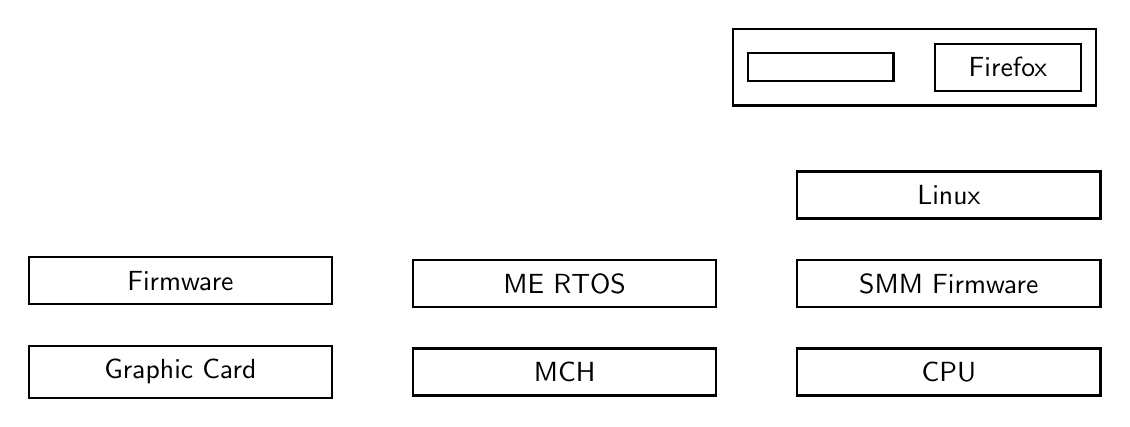
\begin{tikzpicture} [ thick
                    , font=\sffamily
                    , box/.style={text width=3.5cm, inner sep=5pt, text badly centered}
                    , sbox/.style={text width=1.5cm, inner sep=5pt, text badly centered}
                    ]

  % --- Graphic Card Stack ----------------------------------------------------
  \node [ draw
        , box
        ]
        (GC) {Graphic Card};

  \node [ draw
        , box
        , above=0.5cm of GC
        ]
        (GCFW) {Firmware};
  % ---------------------------------------------------------------------------

  % --- MCH/ME Stack ----------------------------------------------------------
  \node [ draw
        , box
        , right=of GC
        ]
        (MCH) {MCH};

  \node [ draw
        , box
        , above=0.5cm of MCH
        ]
        (ME) {ME RTOS};
  % ---------------------------------------------------------------------------

  % --- Main CPU Stack --------------------------------------------------------
  \node [ draw
        , box
        , right=of MCH
        ]
        (CPU) {CPU};

  \node [ draw
        , box
        , above=0.5cm of CPU
        ]
        (CPUFW) {SMM Firmware};

  \node [ draw
        , box
        , above=0.5cm of CPUFW
        ]
        (CPUOS) {Linux};

  \node [ draw
        , sbox
        , above=of CPUOS
        , xshift=0.75cm
        ]
        (A1) {Firefox};

  \node [ draw
        , sbox
        , left=0.5cm of A1
        ]
        (A2) {};

  \node [ draw
        , box
        , fit=(A1) (A2)
        ]
        (Apps) {};

  % ---------------------------------------------------------------------------
\end{tikzpicture}
\end{document}
